\section{Results}\label{sec:results}

We report the results along the chain, and each statistic belongs to one surface of Table~\ref{tab:surfaces}. Everything computed against the Wave~7 file is retrospective. Exact values are in the text, Table~\ref{tab:checks} and the online supplement.

\subsection{Anchor to instrument: what training installs}\label{sec:res-recovery}

Every training pair of a country carries a label. The chosen completion is the one that goes with the sign of the country's GPS coordinate on the pair's own dimension. The first question is whether that installation carries over to pairs the adapters never saw. This is a construction check on the synthetic labels (descriptive, no human data). We split the training pairs once into a training part and a held-out part that the adapters never saw. Recovery is the share of held-out pairs on which the adapter favors the chosen completion more than the base model does, and accuracy is the share on which it prefers that completion outright. Definitions and gates are in the online supplement.

Recovery is \cl{0.940}{C9_label_recovery_recovery_profile_block} \ci{0.926}{0.952}{C9_label_recovery_recovery_profile_block} and accuracy is \cl{0.816}{C9_label_recovery_accuracy_profile_block} \ci{0.771}{0.856}{C9_label_recovery_accuracy_profile_block}. The base model's accuracy is \cl{0.489}{C9_label_recovery_base_accuracy_profile_block} \ci{0.471}{0.506}{C9_label_recovery_base_accuracy_profile_block}. That interval includes one half, so the base model shows no detectable preference for the chosen completions before training. The mean margin shift is \cl{40.3}{C9_label_recovery_mean_margin_shift_profile_block} \ci{28.2}{54.1}{C9_label_recovery_mean_margin_shift_profile_block} nats. Training installs each country's synthetic labels on scenarios the adapter never saw, which is construction fidelity. It says nothing about whether the labels order countries like the GPS, and nothing about respondents. Notably, the distance results below show that the same adapters lie farther from the survey's response distributions than the base model does.

\subsection{Anchor to instrument: the trust order and what carries it}\label{sec:res-bank}

The first cohort encodes four of the six declared signs on the strict battery (S1). Over the \dc{42}{countries} countries, the adapter--GPS Spearman correlation is \cl{0.744}{B2_cohort1_trust_rho} \ci{0.500}{0.865}{B2_cohort1_trust_rho} for trust and \cl{0.435}{B2_cohort1_risktaking_rho} \ci{0.085}{0.686}{B2_cohort1_risktaking_rho} for risk taking. It is \cl{0.488}{B2_cohort1_posrecip_rho} \ci{0.120}{0.695}{B2_cohort1_posrecip_rho} for positive reciprocity and \cl{0.406}{B2_cohort1_altruism_rho} \ci{0.020}{0.676}{B2_cohort1_altruism_rho} for altruism. These four form the imprint set that the screen later uses.

The second cohort tests whether the order survives a change of scenario text (S2). Trust keeps its agreement with the GPS, at \cl{0.803}{B2_bank2_trust_rho} \ci{0.615}{0.876}{B2_bank2_trust_rho}. The other three imprint dimensions keep positive point estimates, but their intervals now include zero (Table~\ref{tab:checks}). Therefore, \cl{1}{B2_n_imprint_kept} of the \cl{4}{B2_n_imprint_kept:n} imprint dimensions passes the second-bank check and \cl{3}{B2_n_imprint_dropped} do not. Under the rule fixed before the second cohort was trained, we write no sentence about the other three carrying over. Trust is the dimension on which retention of the anchor's order is replicated across scenario banks. The banks also agree profile by profile. Over the \dc{26}{profiles_realized} shared profiles, the rank correlation between first-bank and second-bank trust composites is \cl{0.907}{B2_bank_to_bank_trust_spearman} \ci{0.774}{0.957}{B2_bank_to_bank_trust_spearman}. Risk taking is the least stable surface, at \cl{0.544}{B2_bank_to_bank_risktaking_spearman} \ci{0.187}{0.772}{B2_bank_to_bank_risktaking_spearman}, which fits its loss on the second bank (the online supplement gives every surface). This agreement measures how much the scenario text changes the instrument and says nothing about people.

What carries the trust order? The comparison a survey researcher would reach for first is a prompt that names the population. It does not reproduce the order (P): the persona--GPS correlation over the \dc{42}{countries} countries is \cl{0.028}{PX_persona_trust_rho} \ci{-0.339}{0.381}{PX_persona_trust_rho}. The planned contrast with the first cohort is \cl{0.716}{PX_D_cohort1_trust} \ci{0.191}{1.154}{PX_D_cohort1_trust}, and the reading is the same under a country bootstrap. A prompt that states the same six signs in words, with no adapter and no country name, tracks trust as closely as the adapters do. It reaches \cl{0.773}{PX_signprompt_trust_rho} \ci{0.584}{0.844}{PX_signprompt_trust_rho} (panel A of Figure~\ref{fig:route}, which sets all routes side by side). That is, on trust what separates the routes is whether the declared sign is supplied, whichever channel carries it. The contrast sets declared signs against a country name and says nothing about trained weights against prompting. On the other surfaces the persona route's intervals include zero, except for patience, which it orders positively on one item and negatively on the other (online supplement).

\subsection{Inside the instrument: the sign-profile factorial}\label{sec:res-factorial}

The factorial asks whether the six declared signs behave as separate inputs (F). On the trained route, every sign bit moves its own surface in the intended direction (panel A of Figure~\ref{fig:factorial}; the online supplement gives each effect with its $t$ statistic). All seven own effects are positive, from \cl{0.364}{FX_adapter64_trust_own_beta} for trust ($t=\cl{16.74}{FX_adapter64_trust_own_t}$) to \cl{0.124}{FX_adapter64_posrecip_own_beta} for positive reciprocity ($t=\cl{3.02}{FX_adapter64_posrecip_own_t}$), and \cl{0}{FX_adapter64_own_effects_wrong_signed} of \cl{7}{FX_adapter64_own_effects_wrong_signed:n} point the wrong way.

The planned separability check fails. Only \cl{2}{FX_adapter64_V5_hits} of the \cl{6}{FX_adapter64_V5_hits:n} bits move their own surface more than any other surface, where at least \dc{4}{v5_required} were required (binomial $p=\cl{0.207}{FX_adapter64_V5_p_binomial}$). They are the bits for altruism and negative reciprocity. Scale-free views agree (online supplement). Each bit moves its own surface and also moves others, often by more. The risk-taking bit moves the altruism surface by \cl{0.983}{FX_adapter64_risktaking_bit_on_altruism}, against the altruism bit's own effect of \cl{0.242}{FX_adapter64_altruism_own_beta}. The trust bit is the largest mover on \cl{3}{FX_adapter64_surfaces_largest_mover_is_trust_bit} of the \cl{7}{FX_adapter64_surfaces_largest_mover_is_trust_bit:n} surfaces. One common direction carries \cl{51.3}{FX_adapter64_pc1_share:pct}\% of the variance of the seven standardized surfaces, and the mean absolute correlation between surfaces is \cl{0.395}{FX_adapter64_mean_abs_inter_surface_r}. In other words, each sign keeps its intended direction on its own surface, while the size of its effects spreads across the others.

The prompted route fails the check by the same count, \cl{2}{FX_signprompt64_V5_hits} of \cl{6}{FX_signprompt64_V5_hits:n} (binomial $p=\cl{0.207}{FX_signprompt64_V5_p_binomial}$), so V5 does not separate the routes. What separates them is the common direction and the sign of the own effects. Under prompting the first principal component carries \cl{83.5}{FX_signprompt64_pc1_share:pct}\% of the variance, the mean absolute correlation between surfaces is \cl{0.807}{FX_signprompt64_mean_abs_inter_surface_r}, and the trust bit is the largest mover on all \cl{7}{FX_signprompt64_surfaces_largest_mover_is_trust_bit} surfaces. Three prompted own effects point against the intended direction. Two are risk taking at \cl{-0.457}{FX_signprompt64_risktaking_own_beta} ($t=\cl{-22.31}{FX_signprompt64_risktaking_own_t}$) and patience Q43 at \cl{-0.069}{FX_signprompt64_patience_Q43_own_beta} ($t=\cl{-19.75}{FX_signprompt64_patience_Q43_own_t}$). The third, negative reciprocity at \cl{-0.023}{FX_signprompt64_negrecip_own_beta}, is not distinguishable from zero at $t=\cl{-1.80}{FX_signprompt64_negrecip_own_t}$. These are behavioral cross effects of the instrument. The contrast concerns entanglement and the direction of own effects and is silent on screening accuracy, where the difference between routes is unresolved.

\begin{figure}[p]
\centering
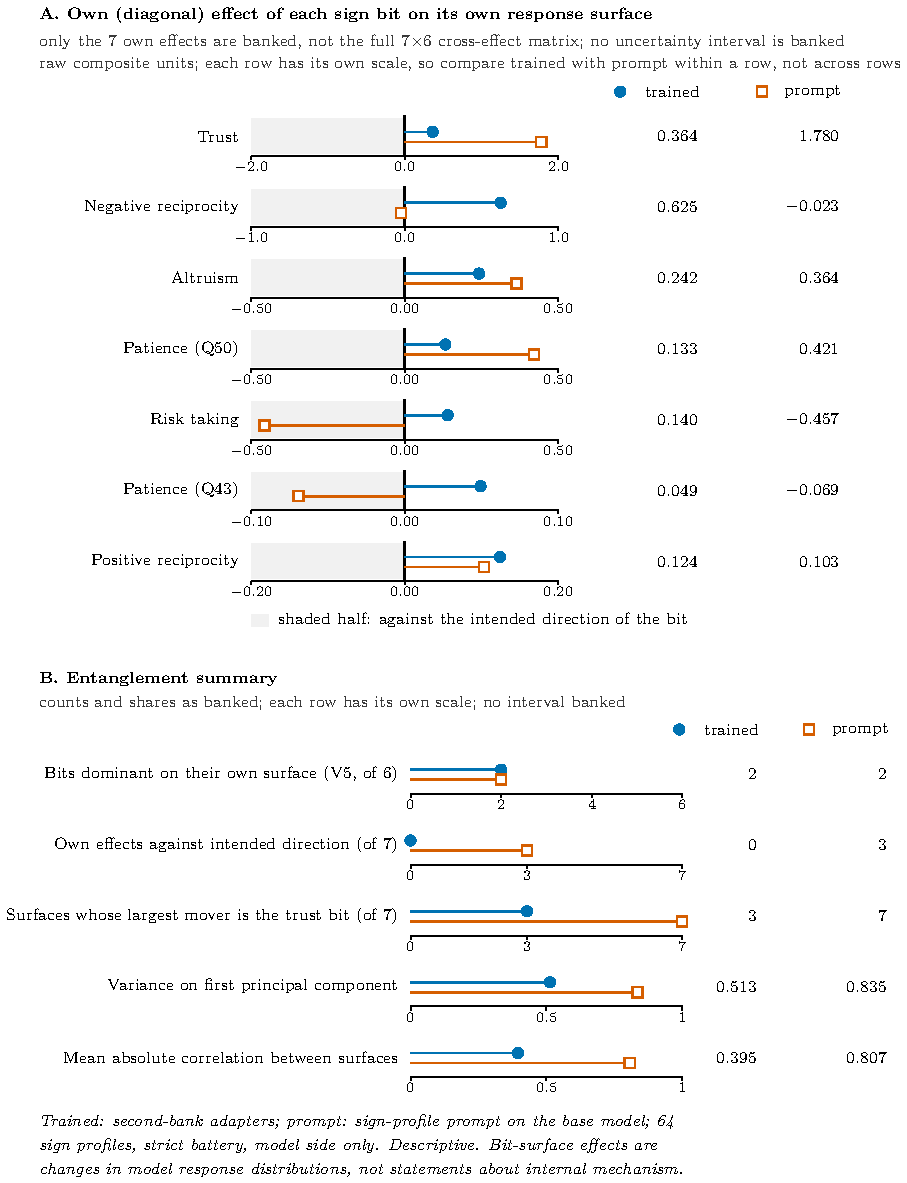
\includegraphics[width=0.91\textwidth]{figures/fig_factorial_own.pdf}
\caption{Own effects of the sign bits in the sixty-four-profile factorial (surface F; model side only). (A) For each of seven strict-battery surfaces, the main effect of the surface's own sign bit, for the trained second-cohort adapters (circles) and the sign-profile prompt (squares). All \cl{7}{FX_adapter64_own_effects_wrong_signed:n} trained own point estimates have the intended sign, and \cl{3}{FX_signprompt64_own_effects_wrong_signed} prompted ones do not. (B) Counts and shares that summarize entanglement. V5 was a planned check; the other rows are exploratory.}\label{fig:factorial}
\end{figure}

We next ask why the trust order survives when the other surfaces lose theirs. We split the second-cohort adapters' main effects into two parts: the effect of each surface's own bit and the summed effect of the other five. We evaluate each part at the sign profile of each of the \dc{42}{countries} countries and correlate it with the GPS coordinate of the surface's own dimension (D; the online supplement gives every surface). This is a behavioral decomposition that uses model quantities and published GPS values only. It says nothing about what happens inside the network. The own-bit part orders the countries like the GPS on all seven surfaces, with correlations from \cl{0.817}{C9_W1_patience_Q43_spearman_own_vs_gps} to \cl{0.866}{C9_W1_posrecip_spearman_own_vs_gps}. That ordering is mechanical. For a positive own effect, as all seven are, the own part is proportional to the sign of the GPS coordinate. It therefore restates the correlation between signs and GPS and is no separate test of learning. The full prediction, which adds the cross bits, keeps the GPS order on trust at \cl{0.834}{C9_W1_trust_spearman_full_vs_gps} and loses most of it elsewhere. On the other surfaces its correlations run from \cl{-0.020}{C9_W1_patience_Q43_spearman_full_vs_gps} for patience Q43 to \cl{0.422}{C9_W1_altruism_spearman_full_vs_gps} for altruism. The cross part carries little of the full prediction's variation on trust and most of it elsewhere. Var(cross)/Var(full) is \cl{0.147}{C9_W1_trust_cross_var_share} on trust and runs from \cl{0.830}{C9_W1_negrecip_cross_var_share} to \cl{1.049}{C9_W1_patience_Q43_cross_var_share} on the other six. This is a ratio of variances and no percentage of variance explained. It exceeds one on patience Q43 because the own and cross parts covary negatively. The comparison sets trust against six surfaces, so it is no graded relation and we claim no dose--response. No bank label depends on a second dimension. In both banks all \cl{27{,}636}{C9_W1_bank1_label_rows_checked} country-pair training rows follow the sign of the pair's own dimension, with \cl{0}{C9_W1_bank1_label_mismatches} mismatches in the first bank and \cl{0}{C9_W1_bank2_label_mismatches} in the second. Therefore, the labels do not carry the cross talk. We claim no cause of the loss, which would need component-level analysis and interventions.

Retraining noise is small beside these effects: an unseeded retrain of one profile moves every strict surface by at most \cl{0.112}{RP_max_abs_surface_diff_sd} of a standard deviation across profiles (R; online supplement). This is a narrow observed comparison of one retrained unit with its original. We did not measure variation across units.\footnote{The near-zero filter (N) is not promoted under the predeclared rule, and two refits support no claim of a reversal across countries. The online supplement gives the margin in full.}

\subsection{Instrument to respondents: the retrospective screen}\label{sec:res-screen}

Retrospectively, the screen rejects its registered null (H). The probe selected \cl{56}{SCR_A_primary:n} of the \dc{223}{pool_items} pool items under the primary rule. Their mean signed agreement with the Wave~7 country differences is $A=\cl{0.061}{SCR_A_primary}$ (Figure~\ref{fig:screen}, panel A), with a country-bootstrap interval of \ci{-0.007}{0.126}{SCR_A_primary}. The permutation null reassigns the same dimension and sign pairs to items drawn at random from the pool. Its distribution has mean \cl{0.012}{SCR_null_mean} and ninety-fifth percentile \cl{0.046}{SCR_null_q95}, and the one-sided $p$ is \cl{0.010}{SCR_p_perm} (panel B).

By the registered reading, the signal is weak. Two WVS waves agree with each other on the selected items fielded in both waves with a mean Spearman correlation of \cl{0.746}{SCR_ceiling_mean} (median \cl{0.767}{SCR_ceiling_median}, \cl{34}{SCR_ceiling_mean:n} items). The screen's $A$ is \cl{8.1}{SCR_A_over_ceiling:pct}\% of that ceiling, well below the registered bar of one third, which would be \cl{0.249}{SCR_one_third_ceiling}. The interval reaches zero while the permutation test rejects the null, because the two answer different questions. The test asks whether the assignments beat random assignments of the same pairs to items from the same pool. The interval asks how much $A$ varies across samples of countries. The direction of the finding is clearer than its size. The registered reliability checks point the same way. The secondary rule gives $A=\cl{0.070}{SCR_secondary_A}$ over \cl{185}{SCR_secondary_A:n} items with a one-sided permutation $p\cl{<0.001}{SCR_secondary_p_perm}$, and dropping one country at a time moves the primary $A$ only between \cl{0.051}{SCR_loco_min} and \cl{0.072}{SCR_loco_max}.

\begin{figure}[p]
\centering
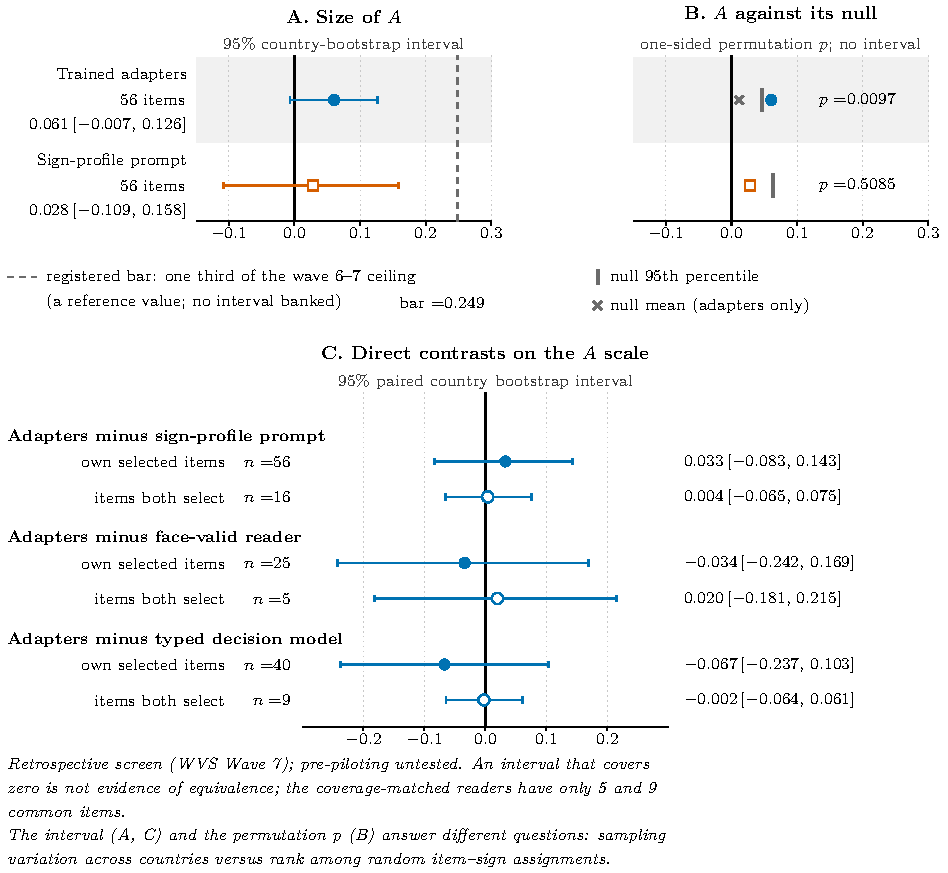
\includegraphics[width=\textwidth]{figures/fig_screen.pdf}
\caption{The retrospective held-out screen (surface H; preregistered, retrospective criterion). $A$ is the mean signed agreement, over the selected items, between the direction the probe assigned to an item and the WVS Wave~7 country differences on that item. (A) $A$ for the \cl{56}{SCR_A_primary:n} items the adapters selected and for the sign-profile prompt's own selection, with \dc{95}{ci_level}\% country-bootstrap intervals over \dc{42}{countries} countries; the dashed line is the registered bar of one third of the two-wave human ceiling, a reference value with no interval. (B) The same $A$ against its permutation null: the bar is the null's ninety-fifth percentile, the cross its mean (adapters only; none is banked for the prompt), and the one-sided $p$ is printed. (C) Paired contrasts, adapters minus each comparator, on each route's own items and on items both select ($n$ printed), with \dc{95}{ci_level}\% paired country-bootstrap intervals; the registered primary contrasts are those with questionnaire readers on shared items. Interval and permutation $p$ answer different questions, and an interval covering zero is not evidence of equivalence.}\label{fig:screen}
\end{figure}

The per-dimension readings show where the signal sits (Table~\ref{tab:checks}). Under the primary rule, only the items assigned to risk taking have an interval above zero. Their $A_d=\cl{0.158}{PD_adapter_primary_risktaking_A}$ \ci{0.015}{0.290}{PD_adapter_primary_risktaking_A} on \cl{13}{PD_adapter_primary_risktaking_A:n} items, of which \cl{92.3}{PD_adapter_primary_risktaking_share_pos:pct}\% agree in sign. The intervals for trust and altruism include zero. The items assigned to positive reciprocity point the wrong way: their point estimate is negative, and only \cl{18.2}{PD_adapter_primary_posrecip_share_pos:pct}\% of the \cl{11}{PD_adapter_primary_posrecip_share_pos:n} items agree in sign. Under the exploratory Bonferroni adjustment for four dimensions, the interval for risk taking becomes \ci{-0.026}{0.326}{PD_adapter_primary_risktaking_A_bonf} and includes zero.\footnote{The probe's per-dimension permutation $p$ values were not registered. For altruism under the primary rule they point the other way from the registered interval, so we report the registered intervals only.}

% Table 2: both checks per imprint dimension. Every number is a \cl / \ci macro tied to NUMBERS_TABLE.csv.
\begin{table}[htbp]
\centering
\caption{The second-bank check and the retrospective screen, by imprint dimension. The two checks are reported side by side and never averaged.}\label{tab:checks}
\small
\renewcommand{\arraystretch}{1.2}
\begin{tabularx}{\textwidth}{@{}>{\raggedright\arraybackslash}p{0.17\textwidth}>{\raggedright\arraybackslash}X>{\raggedright\arraybackslash}X>{\raggedright\arraybackslash}X>{\raggedright\arraybackslash}X@{}}
\toprule
 & S2: second bank & H: primary rule & H: primary rule, Bonferroni & H: secondary rule \\
Dimension & $\rho$ [\dc{95}{ci_level}\% interval] & $A_d$ [\dc{95}{ci_level}\% interval], items & $A_d$ [adjusted interval] & $A_d$ [\dc{95}{ci_level}\% interval], items \\
\midrule
Trust & \cl{0.803}{B2_bank2_trust_rho} \newline \ci{0.615}{0.876}{B2_bank2_trust_rho}
 & \cl{0.062}{PD_adapter_primary_trust_A} \newline \ci{-0.047}{0.173}{PD_adapter_primary_trust_A}, \cl{12}{PD_adapter_primary_trust_A:n}
 & \ci{-0.088}{0.199}{PD_adapter_primary_trust_A_bonf}
 & \cl{0.092}{PD_adapter_secondary_trust_A} \newline \ci{-0.019}{0.199}{PD_adapter_secondary_trust_A}, \cl{44}{PD_adapter_secondary_trust_A:n} \\
Risk taking & \cl{0.210}{B2_bank2_risktaking_rho} \newline \ci{-0.199}{0.584}{B2_bank2_risktaking_rho}
 & \cl{0.158}{PD_adapter_primary_risktaking_A} \newline \ci{0.015}{0.290}{PD_adapter_primary_risktaking_A}, \cl{13}{PD_adapter_primary_risktaking_A:n}
 & \ci{-0.026}{0.326}{PD_adapter_primary_risktaking_A_bonf}
 & \cl{0.143}{PD_adapter_secondary_risktaking_A} \newline \ci{0.045}{0.229}{PD_adapter_secondary_risktaking_A}, \cl{50}{PD_adapter_secondary_risktaking_A:n} \\
Positive reciprocity & \cl{0.366}{B2_bank2_posrecip_rho} \newline \ci{-0.068}{0.652}{B2_bank2_posrecip_rho}
 & \cl{-0.071}{PD_adapter_primary_posrecip_A} \newline \ci{-0.281}{0.154}{PD_adapter_primary_posrecip_A}, \cl{11}{PD_adapter_primary_posrecip_A:n}
 & \ci{-0.332}{0.205}{PD_adapter_primary_posrecip_A_bonf}
 & \cl{-0.049}{PD_adapter_secondary_posrecip_A} \newline \ci{-0.198}{0.117}{PD_adapter_secondary_posrecip_A}, \cl{22}{PD_adapter_secondary_posrecip_A:n} \\
Altruism & \cl{0.364}{B2_bank2_altruism_rho} \newline \ci{-0.057}{0.653}{B2_bank2_altruism_rho}
 & \cl{0.069}{PD_adapter_primary_altruism_A} \newline \ci{-0.036}{0.177}{PD_adapter_primary_altruism_A}, \cl{20}{PD_adapter_primary_altruism_A:n}
 & \ci{-0.058}{0.198}{PD_adapter_primary_altruism_A_bonf}
 & \cl{0.040}{PD_adapter_secondary_altruism_A} \newline \ci{-0.038}{0.117}{PD_adapter_secondary_altruism_A}, \cl{69}{PD_adapter_secondary_altruism_A:n} \\
\bottomrule
\end{tabularx}
\par\smallskip
\begin{minipage}{\textwidth}\footnotesize
\textit{Note:} S2 is the Spearman correlation between second-bank adapter composites and the GPS coordinate over \dc{42}{countries} countries, with a profile-block bootstrap (\dc{2,000}{boot_draws} draws, seed \dc{20261011}{seed_c3}); model side only. H is the retrospective screen against WVS Wave~7 country means: $A_d$ is the mean signed item agreement over the selected items assigned to the dimension, with the registered country bootstrap (\dc{2,000}{boot_draws} resamples, seed \dc{20261015}{seed_screen}). The registered intervals are unadjusted; the Bonferroni intervals over the \dc{4}{imprint_dims} imprint dimensions are exploratory and read off the same draws. The secondary rule is a registered reliability check. No dimension has an interval above zero on both S2 and H.
\end{minipage}
\end{table}


The two checks disagree by dimension. Trust survives the second bank, and its screen interval includes zero. Risk taking is the one dimension whose screen interval excludes zero before adjustment, and it is one of the three that lose their interval on the second bank. No dimension passes both registered checks, and the per-dimension cells are small.

\subsection{Instrument to respondents: questionnaire readers and the prompt route}\label{sec:res-comparators}

The registered contrasts do not distinguish the adapters from a careful reader of the questionnaire (Figure~\ref{fig:screen}, panel C; the online supplement tabulates every contrast). Every interval covers zero, which the preregistration reads as ``the adapters match a careful reader''. That reading rests on few items. The coverage-matched contrasts use the \cl{5}{CMP_face_valid_D_common:n} items that the adapters and the face-valid rule both assign and the \cl{9}{CMP_jev_D_common:n} items they share with the typed decision model. The routes agree on dimension and sign for \cl{1}{CMP_face_valid_common_same_dim_sign} and \cl{7}{CMP_jev_common_same_dim_sign} of them. An interval that covers zero on so few items is consistent with a match and does not establish one. Both readers concentrate on trust, where their own-item $A$ exceeds the \cl{0.062}{PD_adapter_primary_trust_A} of the adapters' own trust items, but their per-dimension cells are too small to be informative.

Prompting the base model with the same six signs does not pass the registered null. The same probe applied to the \dc{64}{cells} prompted profiles gives $A=\cl{0.028}{SP_A_primary}$ \ci{-0.109}{0.158}{SP_A_primary} with a one-sided permutation $p$ of \cl{0.509}{SP_p_perm}, and it assigns its selected items to a single dimension, trust. The adapter route passes the null and the prompt route does not, but the direct difference between them is unresolved. Adapter minus prompt is \cl{0.033}{SP_D_own} on each route's own items and \cl{0.004}{SP_D_common} on the \cl{16}{SP_overlap_with_adapter} items both select, and both intervals cover zero. The two routes agree on dimension and sign for \cl{6}{SP_overlap_same_dim_sign} of those shared items. We therefore cannot credit the trained weights over the prompt on the screen.

Item-level assignment is stable under option order and paraphrase, whereas membership in the particular selected set churns. The registered statistic is the number of selected items whose dimension and sign are unchanged. It is \cl{39}{RO_heldout_reverse_ds_unchanged} of \cl{56}{RO_heldout_reverse_ds_unchanged:n} with reversed options, \cl{39}{RO_heldout_para_a_ds_unchanged} with the first paraphrase and \cl{30}{RO_heldout_para_b_ds_unchanged} with the second. No variant changes more than half, so the registered condition for wording dependence is not met, although the second paraphrase comes close. Membership is another matter: the primary rule is a top-quartile cut on $|t|$, and only \cl{18}{RO_heldout_reverse_membership_agreement}, \cl{29}{RO_heldout_para_a_membership_agreement} and \cl{16}{RO_heldout_para_b_membership_agreement} of the \cl{56}{RO_heldout_para_b_membership_agreement:n} items are selected under both the original readout and each variant. Dimension and direction are more stable than the list of top-ranked items.

\subsection{Instrument to respondents: agreement with the human composite}\label{sec:res-human}

The next two subsections report descriptive follow-up analyses (D), added after the registered results had been read. None is preregistered and none enters a registered family. They set the instrument beside the respondents of the Wave~7 file on the strict battery, and every statement is retrospective. Figure~\ref{fig:links} gives three Spearman correlations over the \dc{42}{countries} countries for each of seven surfaces. They pair the adapter composite with the GPS, the adapter composite with the human composite of the same items, and the human composite with the GPS. The panels have different statistical targets and bootstrap units, so their widths are not comparable.

\begin{figure}[p]
\centering
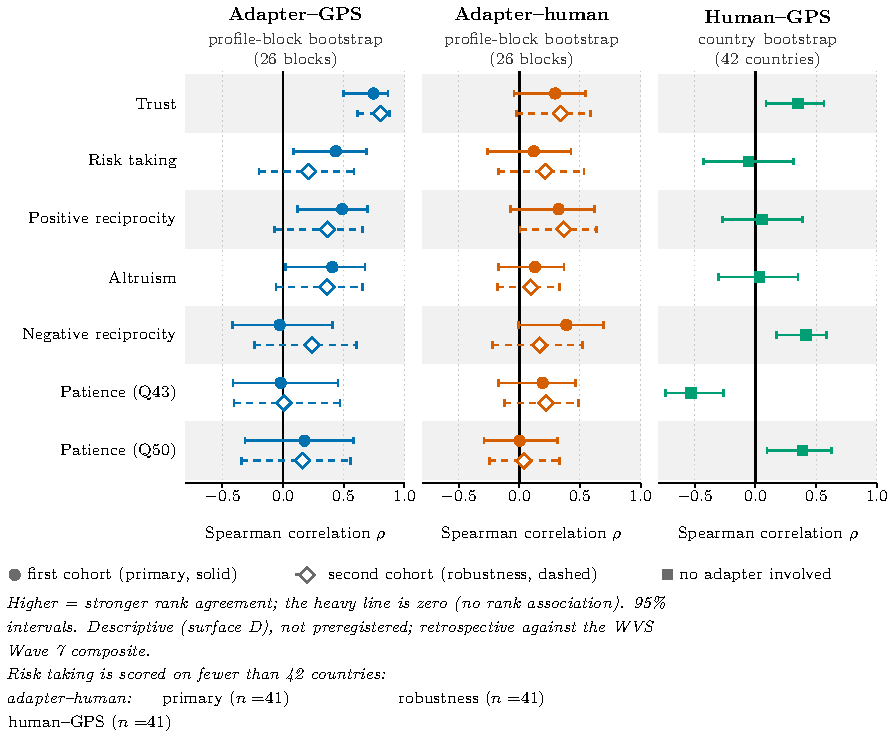
\includegraphics[width=\textwidth]{figures/fig_three_links.pdf}
\caption{The three links on seven strict-battery surfaces (surface D; descriptive, not preregistered; retrospective). Each mark is a Spearman correlation across countries with a \dc{95}{ci_level}\% interval; the heavy line is zero. Left: first-cohort adapter composite with the GPS coordinate of the surface's own dimension. Middle: adapter composite with the Wave~7 composite of the same items. Right: that human composite with the GPS. Circles are first-cohort adapters (primary), diamonds second-cohort adapters (robustness), squares involve no adapter. Intervals in the adapter panels come from a bootstrap over the \dc{26}{profiles_realized} realized sign profiles, those in the right panel from a bootstrap over the \dc{42}{countries} countries. Risk taking covers \cl{41}{C9_a_adapter_human_risktaking_spearman_rho:n} countries in the two human columns.}\label{fig:links}
\end{figure}

On trust, the first-cohort adapters track the GPS at \cl{0.744}{C9_a_adapter_gps_trust_spearman_rho} \ci{0.500}{0.865}{C9_a_adapter_gps_trust_spearman_rho}. They do not detectably reach the human composite, at \cl{0.295}{C9_a_adapter_human_trust_spearman_rho} \ci{-0.044}{0.547}{C9_a_adapter_human_trust_spearman_rho}. All seven adapter--human intervals include zero, which is not evidence that no association exists. The largest point estimate belongs to negative reciprocity, \cl{0.389}{C9_a_adapter_human_negrecip_spearman_rho} \ci{-0.008}{0.694}{C9_a_adapter_human_negrecip_spearman_rho}, a surface on which the adapters do not track the GPS. The second-cohort adapters give the same picture on trust, with an adapter--human correlation of \cl{0.340}{C9_b_adapter_human_trust_spearman_rho} \ci{-0.025}{0.586}{C9_b_adapter_human_trust_spearman_rho}. Positive reciprocity is the one second-cohort interval that excludes zero, and only just (online supplement).

The link between the GPS and the human composite is itself loose on these items. Its interval excludes zero on four of the seven surfaces. Among them, it is positive for trust at \cl{0.351}{C9_a_human_gps_trust_spearman_rho} \ci{0.088}{0.564}{C9_a_human_gps_trust_spearman_rho} and negative for patience Q43 at \cl{-0.533}{C9_a_human_gps_patience_q43_spearman_rho} \ci{-0.741}{-0.266}{C9_a_human_gps_patience_q43_spearman_rho}. We read this column as a reference for scale. It is no upper bound on what an adapter could reach, because it does not bound a scorer that is nonlinear or constant within sign profiles. Nor is it evidence that the anchor limits the instrument. Together, the three panels say that the adapters carry the GPS order on trust and that the GPS order is only loosely related to the human composite. They also show that the adapters' order of countries does not detectably agree with the human composite on any surface. The exact values for every cell are in the online supplement.

\subsection{Instrument to respondents: order versus distance}\label{sec:res-tvd}

The correlations above concern the order of countries. A different question is how far the instrument's response distribution lies from the survey's. We measure it by the country-equal mean total variation distance (TVD; lower is closer; D) in four cells. They are the base model and the first-cohort adapters, each with and without the country-named persona prompt.

The base model's mean distance is \cl{0.470}{C9_TVD_base_mean_tvd_country_equal}. The adapters sit farther from the survey at \cl{0.515}{C9_TVD_adapter_mean_tvd_country_equal}, and the persona prompt sits closer at \cl{0.365}{C9_TVD_persona_mean_tvd_country_equal} (panel B of Figure~\ref{fig:route}). A cell mean carries no interval, whereas the paired contrasts of panel C each carry one. Relative to the base model, the adapters are farther by \cl{0.045}{C9_TVD_adapter_minus_base_profile_block} \ci{0.006}{0.093}{C9_TVD_adapter_minus_base_profile_block} under profile blocks, and the persona prompt is closer by \cl{-0.105}{C9_TVD_persona_minus_base_profile_block} \ci{-0.122}{-0.086}{C9_TVD_persona_minus_base_profile_block}. Country resampling gives the same readings. With both interventions the distance is \cl{0.420}{C9_TVD_adapter_persona_mean_tvd_country_equal}. Adding the persona prompt to the adapters moves the distance by \cl{-0.096}{C9_TVD_adapter_persona_minus_adapter_profile_block} \ci{-0.115}{-0.078}{C9_TVD_adapter_persona_minus_adapter_profile_block}, and adding the adapters to the persona prompt moves it by \cl{0.055}{C9_TVD_adapter_persona_minus_persona_profile_block} \ci{0.016}{0.097}{C9_TVD_adapter_persona_minus_persona_profile_block}. The interaction contrast is the adapters' effect with the persona prompt minus their effect without it. Under profile blocks it is \cl{0.009}{C9_TVD_interaction_profile_block} \ci{-0.003}{0.022}{C9_TVD_interaction_profile_block}, an interval that includes zero. Therefore, the data show no detectable departure from additivity.

\begin{figure}[p]
\centering
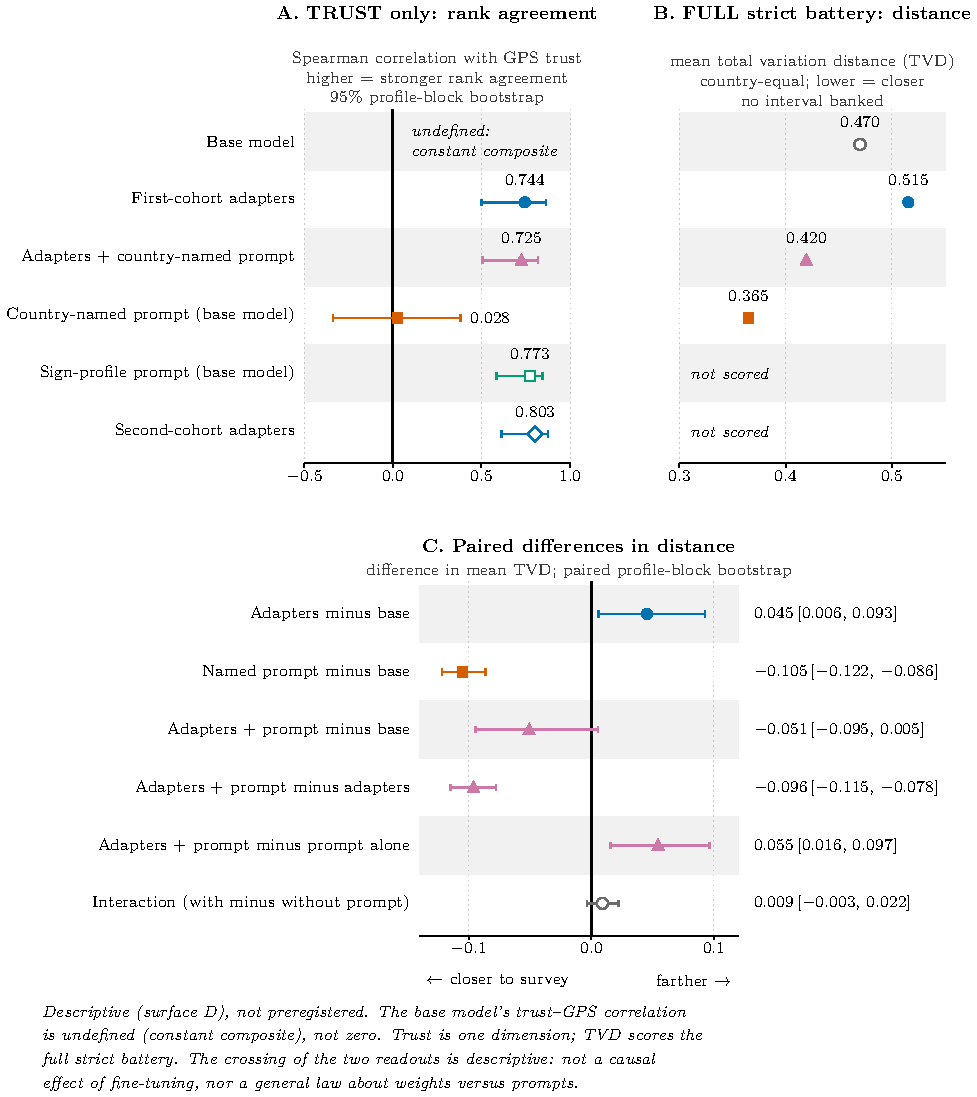
\includegraphics[width=0.98\textwidth]{figures/fig_info_vs_route.pdf}
\caption{Order and distance for the same routes (a descriptive display, not preregistered; the distances are retrospective). (A) Trust only: Spearman correlation of each route's trust composite with the GPS trust coordinate over \dc{42}{countries} countries, with \dc{95}{ci_level}\% profile-block intervals. The first-cohort, second-bank and country-named values are those of Section~\ref{sec:res-bank}, where their own status is stated. (B) Mean total variation distance (TVD) to the survey answer shares over the full strict battery, country-equal; routes not scored on this battery are marked. (C) Paired differences in mean TVD with \dc{95}{ci_level}\% profile-block intervals; negative means the first-named cell is closer. Panel A scores trust only and panels B and C all dimensions, so they are different metrics.}\label{fig:route}
\end{figure}

The ordering of the cells by distance does not follow their ordering by trust agreement with the GPS. The persona prompt has the lowest distance and no trust order (Section~\ref{sec:res-bank}). The adapters have the highest distance and keep the trust order. Adding the persona prompt to the adapters keeps the trust order at \cl{0.725}{C9_TVD_adapter_persona_trust_gps_profile_block} \ci{0.505}{0.820}{C9_TVD_adapter_persona_trust_gps_profile_block} while the distance falls.
